% !TeX spellcheck = french
\documentclass[12pt]{report}

\usepackage[table,xcdraw]{xcolor}

\usepackage[utf8]{inputenc}
\usepackage[T1]{fontenc}
\usepackage[francais]{babel}
\usepackage{fixltx2e}
\usepackage{charter}
\usepackage{amsmath}
\usepackage{float}
\usepackage{wrapfig}
\usepackage{graphicx}
\usepackage{soul}
\usepackage[colorlinks=true, linkcolor=blue]{hyperref}
\usepackage[a4paper, width=150mm, top=25mm, bottom=25mm]{geometry}
\usepackage{parskip}
\usepackage{enumitem}
\usepackage[final]{pdfpages}
%\usepackage{titlesec}
\usepackage{listings}
\usepackage[final]{pdfpages}
\usepackage[font=small,labelfont=bf]{caption} % Required for specifying captions to tables and figures
\setlist[itemize]{label=\textbullet}
\usepackage[linesnumbered,algoruled,french,onelanguage]{algorithm2e}
 \usepackage{url}
\lstset{
	language=Python,                   % choix du langage (de programmation).
	keywordstyle=\color{blue},      % choix de la couleur des mots clés.
	stringstyle=\color{red},        % choix de la couleur des string.
	commentstyle=\color{green},     % choix de la couleur des commentaire.
	basicstyle=\normalsize,     % taille de la police du code
	% numbers=left,                   % placer le numéro de chaque ligne à gauche (on peut choisir à droite, ou ne pas mettre cette option pour aucun numéro de ligne).
	numberstyle=\normalsize,        % taille de la police des numéros.
	numbersep=0pt,                  % distance entre le code et sa numérotation.
	showstringspaces=false,         % pour ne pas afficher les espaces comme des caractères .
	breaklines=true,                % couper la ligne si la ligne du code est trop longue.
}



\begin{document}
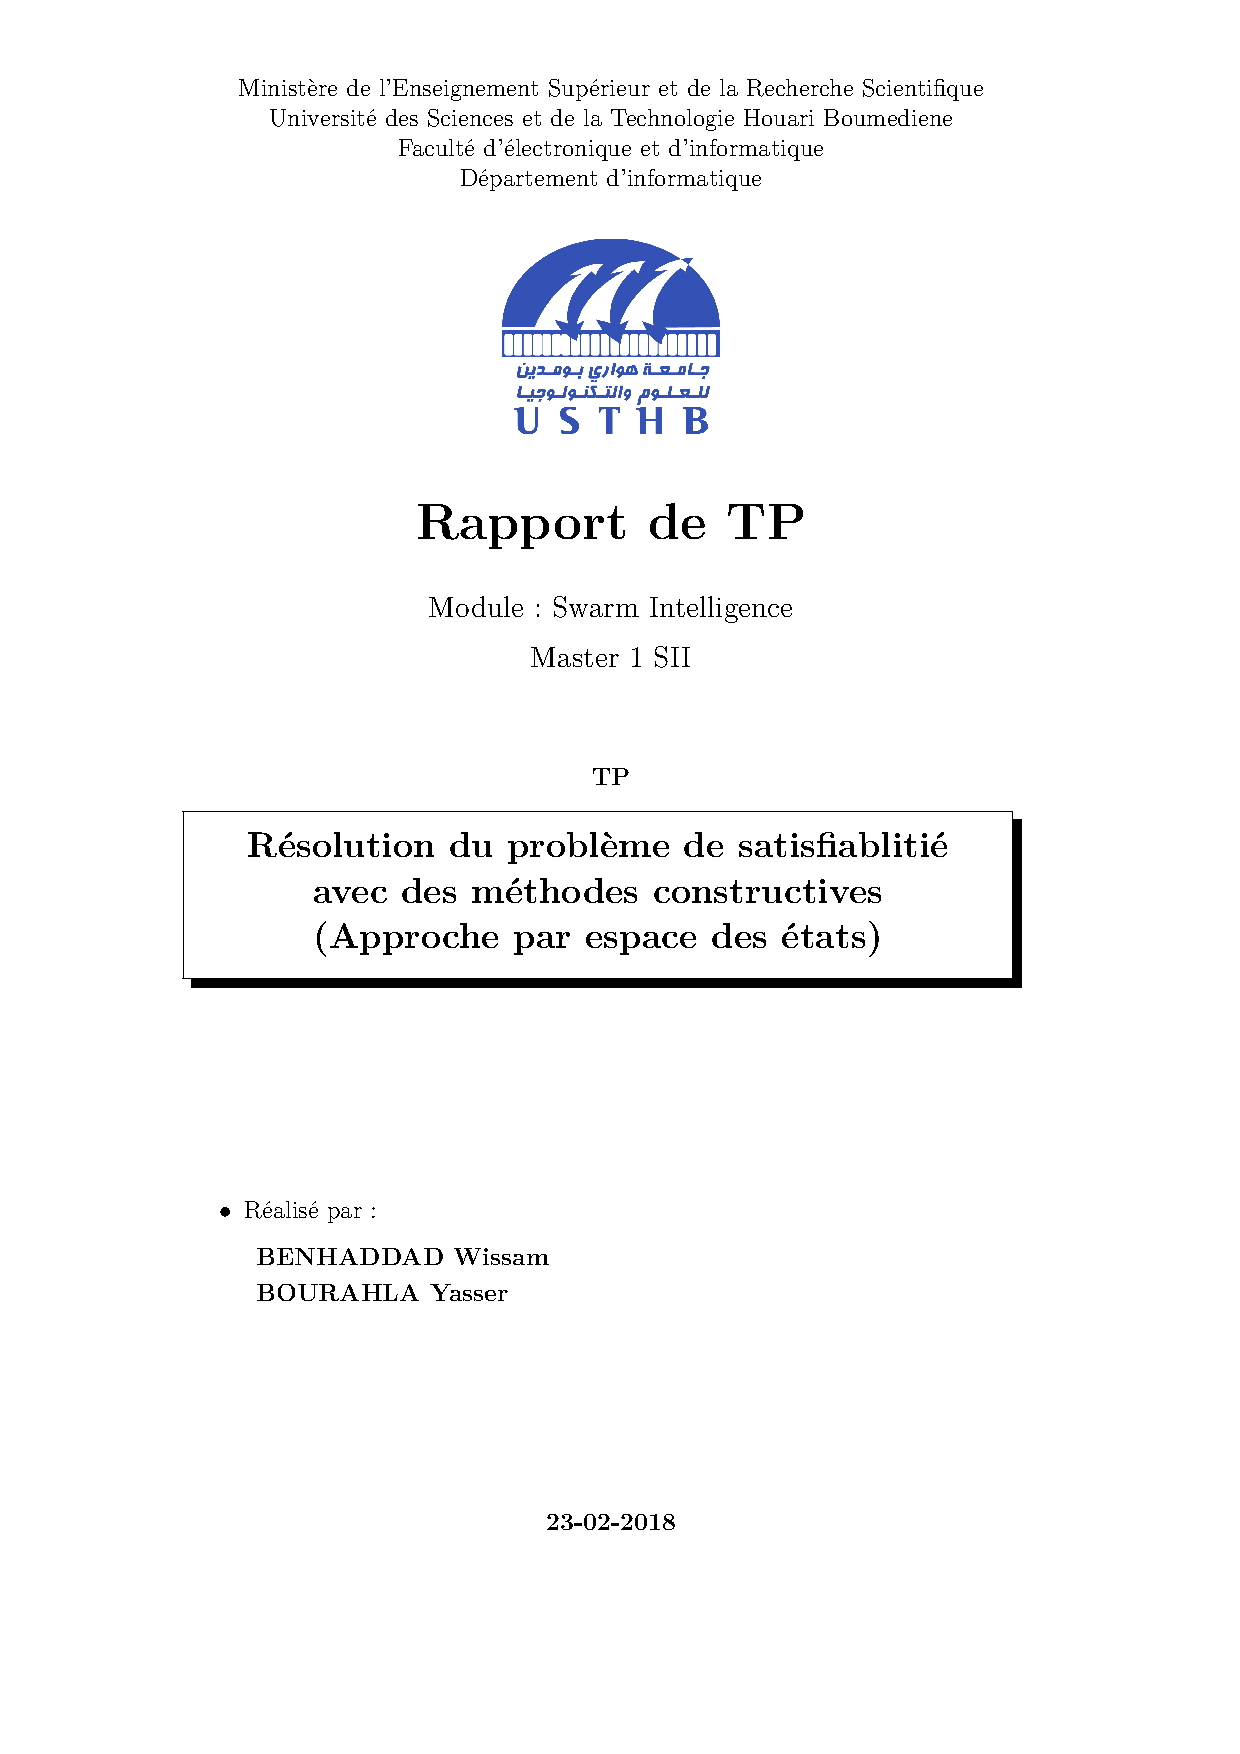
\includepdf[pages=1]{Page_garde.pdf} 
\tableofcontents

\pagenumbering{arabic}
\newpage
\chapter{Introduction : }
\section{Problématique : }
\paragraph{}
Dans ce TP, nous allons tenter d'implémenter et de comparer plusieurs méthodes aveugles, dites aussi \textbf{à base d'espace d'états}, Pour la résolution du problème de satisfiabilité, plus communément appelé \textbf{Problème SAT}, Ce travail est aussi une application directe des différentes méthodes vues durant le premier semestre en ce qui concerne la \textbf{Résolution de problèmes}, mais aussi la \textbf{Complexité des algorithmes et les structures de données}.
\section{Définitions}
\subsection{Problème SAT}
Dans le domaine de l'informatique et de la logique, le problème de satisfiablité (\textbf{SAT}), est un problème de décision ou il s'agit d'assigner des valeurs de vérité à des literaux\footnote{Une variables logique ou bien sa négation} tel qu'un ensembles de clauses en forme normale conjonctives FNC\footnote{Une conjonction de disjonction de litéraux} préalablement défini soit satisfiable, en d'autres termes, que toutes les clauses soient vraies pour les mêmes valeurs de vérité de leurs literaux, ce problème est le premier à avoir été démontré comme étant \textbf{NP-Complet}, et cela par \href{https://en.wikipedia.org/wiki/Stephen_Cook}{Stephen Cook} dans \cite{cook}, et qui a donc posé les fondements de l'informathique théoriques et de la théorie de la complexité.
\newpage
\subsection{Stratégie de recherche dans l'espace des états}
En cosidérant l'espace de recherche comme étant un arbre, dont les noeuds sont les differents états du problème, nous pouvons classer les différentes stratégies de recherches en deux grandes catégories :
\subsection
{Stratégie de rercherche aveugle}
\subsubsection{Par prodonfeur d'abord (DFS)}
\paragraph{}
L'algorithme de parcours en profondeur d'abord consiste a visité un noeud de départ (souvent appelé \textbf{racine}), puis ensuite visite le premier sommet voisin(ou \textbf{successeur}) jusqu'à ce qu'une profondeur limite soit atteinte ou bien qu'il n'y ait plus de voisin à developper, une variante de cet algorithme utilise deux ensemble \textbf{Open} et \textbf{Closed} qui représentent réspectivement l'ensemble des noeuds du graphe qui n'ont pas encore étés developpés et ceux déjà développés, cet ajout permet à l'algorithme d'éviter de boucler indéfiniment sur un ensemble de noeuds.
\subsubsection{En Largeur d'abord (BFS)}
\paragraph{}
Cet algorithme diffère de son prédecesseur par le fait qu'il visite tous les voisins(\textbf{successeurs}) d'un noeud avant de passer au noeud suivant, ce qui revient à gérer l'ajout et la suppression de l'ensemble Open comme une file, donc en mode \textbf{FIFO} (En supposant bien sûr qu'on dispose des deux ensembles open et closed), cet approche permet de sauvegarder tous les noeuds précèdemment visité durant la recherche, ce qui peut causer un débordement de la mémoire lors de l'exécution sur machine(Ce point sera rediscuté dans \ref{tests} )

\subsubsection{Par coût uniforme}
Le principe est simple, au fur et à mesur que l'algorithme avance et développe des noeuds, il garde en mémoire le coût\footnote[1]{Fonction retournant le cout pour passer du noeud de départ(la racine) au noeud courant}, le noeud qui sera ensuite choisi sera celui dont le coût accumulé est le plus bas, assurant ainsi de toujours choisir le chemin le plus optimal, si le coût pour passer d'un noeud à n'importe quel autre de ses voisins est le même quelque soit le neoud, l'algorithme est alors équivalent à celui de la recherche en largeur d'abord
\subsection
{Stratégie de rercherche guidée}
\subsubsection{Recherche gloutonne (Greedy algorithm)}
\paragraph{}
Cet algorithme est basé sur la notion d'heuristique\footnote[1]{Une fonction d'éstimation de la distance séparant le noeud courant au but }, au lieu de parcourir de façon "naïve" l'ensemble des noeuds dans l'espace de recherche, il choisit a chaque itérration sur l'ensemble \textbf{open} le noeud le plus \textbf{prometteur} en terme de distance par rapport au but recherché.
\newpage
\subsubsection{Algorithme A*}
\paragraph{}
Contrairement aux précedents algorithmes de recherche qui effectuaient une recherche de façon "naîve", l'algorithme \textbf{A* }propose une vision un peu nouvelle, il utilise la notion de coût et celle d'heuristique, la fonction d'évaluation $f$ est donc définie comme étant la somme de deux fonctions $g$ et $h$ ou : \\
	\begin{itemize}
		\item $g$ est la fonction  qui retourne le cout d'un noeud $n$
		\item $h$ est la fonction  qui estime le cout d'un noeud $n$ vers le but
	\end{itemize} 
Le principe de l'algorithme est donc de prendre le noeud dans \textbf{open} qui possède la valeur minimal de $f$, assurant ainsi de trouver le chemin optimal \textbf{ssi.} l'heuristique $h$ choisie est admissible\footnote[2]{Ne surestime jamais le coût réel pour atteindre le but, elle est \textbf{optimiste}}


\newpage
\chapter{Implémentation}
\section{Structures de données}
\section{Conception et pseudo-code}
\subsection{Profondeur d'abord}
\subsection{Largeur d'abord}
\subsection{Recherche gloutonne }
\subsection{Algorithme A*}


\newpage
\chapter{Expérimentations}
\section{Donnés}\label{dataSet}
\paragraph{}
\newpage
\section{Environement de travail}
\subsection{Machines}
\paragraph{}
Pour les tests nous avons utilisé deux machines pour chaques groupes d'instances, autrement dit une machine pour éffecutuer les tests sur un ensembles d'instances satisfiables \textbf{UF75-325}\cite{Benchmark} et une autre sur les instances contradictoires(non satisfiables) \textbf{UUF75-325}\cite{Benchmark}, les caractéristiques de chaques machines sont données dans les figures \ref{fig:machineA} et \ref{fig:machineB} suivantes : 
\begin{figure}[H]
	\centering
	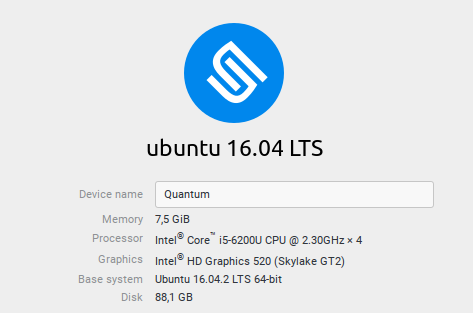
\includegraphics[scale=0.75]{images/machineWISS.png}
	\caption{Machine \textbf{A} pour les instances contradictoires}
	\label{fig:machineA}
\end{figure}
\begin{figure}[H]
	\centering
	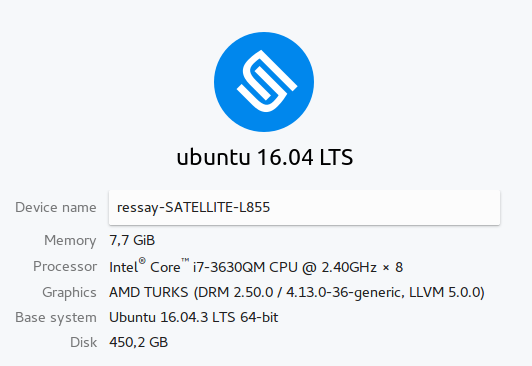
\includegraphics[scale=0.665]{images/machineYASSER.png}
	\caption{Machine \textbf{B} pour les instances satisfiables}
	\label{fig:machineB}
\end{figure}
\newpage
\subsection{Outils utilisés}
\subsubsection{Langage de programmation : }
\paragraph{}

\subsubsection{IDE : }
\paragraph{}
\paragraph{IntelliJ Idea} L'environement de dévelopement choisit est \href{URL}{IntelliJ IDEA}, spécialement dédié au développement en utilisant le langage \href{URL}{JAVA}, il est proposé par l'entreprise \href{https://www.jetbrains.com}{JetBrains} il est caractérisé par sa forte simplicité d'utilisation et les nombreuse plugins et extentions qui lui sont dédiées.

\section{Résultats}\label{tests}
\paragraph{}
\section{Statistiques}
\paragraph{}
\section{Comparaison entres les quatres méthodes}
\paragraph{}

\chapter{Conclusion}
\listoffigures
\bibliographystyle{unsrt}
\bibliography{biblio.bib}
\end{document}}